I have chosen to solve this using the bisection method. I decided the easiest way to do this was by implementing it in python. It is included as a function named "bisect" in the Q0020.py file.\\
With this script we can clearly see that the bisection method converges on a solution significantly more slowly than the secant method. An advantage of both of these functions is that they do not need to calculate the derivative of the function in question. This is useful when finding that derivative is computationally expensive.
\begin{figure}[ht]
  \centering
  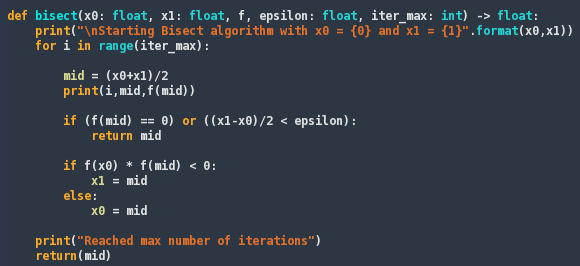
\includegraphics[width = \linewidth]{code.png}
  \caption{The code for implementing the bisection method}
\end{figure}
